\documentclass[12pt]{article}

% Packages for Times New Roman font
\usepackage{times}
\usepackage{mathptmx} % For Times New Roman math font
\renewcommand{\familydefault}{\rmdefault} % Ensures Times New Roman is used throughout

% Additional useful packages
\usepackage[margin=1in]{geometry} % Page margins
\usepackage{setspace} % For line spacing control
\usepackage{graphicx} % For including images
\usepackage{amsmath} % For mathematical equations
\usepackage{cite} % For citations
\usepackage{hyperref} % For hyperlinks in PDF
\usepackage{booktabs} % For professional tables
\usepackage{caption} % For customizing captions

% Document setup - font size enforcement and single spacing
\AtBeginDocument{\fontsize{12pt}{14.4pt}\selectfont} % Enforces 12pt font size throughout
\singlespacing % Set to single spacing as requested
% Use \onehalfspacing or \doublespacing if different spacing is required

% Removed section numbers
\setcounter{secnumdepth}{0}

% Title information
\title{A Hybrid ACO-Reinforcement\\Learning Framework for Task Assignment}
\author{
	Sampath Kumar\\
	\texttt{sz4961@srmist.edu.in}\\
	Department of Computer Science Engineering\\SRM Institute of Science and Technology\\Chennai, India
	\and
	Dr.Krishnaraj N\\
	\texttt{krishnan2@srmist.edu.in}\\
	Department of Networking And Communications\\SRM Institute of Science and Technology\\Chennai, India
}
\date{\today}

\begin{document}
	
	\maketitle
	
	\begin{abstract}
		This paper presents a new approach on combining Ant Colony Optimization (ACO)
		with Reinforcement Learning (RL) techniques employing Q-learning and SARSA,
		to organize and allocate tasks in complex work environments. This approach addresses
		issues with order of task execution, diverse employee skills, employee availability,
		and fair workload distribution. ACO creates an initial task sequence considering
		dependencies and deadlines. Using the ACO determined task sequence, RL agents
		determine the initial assignments by basing their decisions depending on skill
		fit, workload distribution along with deadlines. This approach uses a multi objective
		hyperparameter tuning with Optuna library to balance high rate of task assignment
		with workload distribution."Refinement RL" component provides final passthrough
		by balancing the workload across the skills to ensure employees are not overloaded.
		Experiments reveal that in task assignment rate and workload distribution, the
		ACO-RL combination performs better than simple greedy approach. This study
		adds to ongoing research on scheduling and task assignment optimization
		problems in complex industrial setups.
	\end{abstract}
	
	\section{\label{sec}Introduction}
	Task assignment in industrial settings presents significant challenges due to constraints on employees, hours, skills, and efficiency. Traditional rule-based scheduling methods fail in dynamic environments with uncertainties like machine failures and changing market demands\cite{zhang2022, li2024}.
	\subsection{\label{subsec}Challenges Across Sectors}
	This problem affects various sectors: factories need scheduling to prevent delays and costs; hospitals must meet patient needs while managing staff constraints; tech teams require flexibility for project changes; and call centers must maintain service despite varying demand.
	\subsection{\label{subsec}Impact of Remote Work}
	Remote work has further complicated scheduling by introducing considerations of time zones, employee availability, project sharing, skills, and attrition. Conventional "first come first assign" methodologies are inadequate for modern business dynamics\cite{wang2023}.
	\subsection{\label{subsec}Proposed Hybrid Approach}
	This study proposes a framework (Fig.~\ref{fig:flow}) combining Reinforcement Learning and Ant Colony Optimization. The approach consists of: (1) task sequencing via ACO to satisfy dependencies and restrictions; (2) initial employee assignment using Q-learning and SARSA with reward shaping based on skills, deadlines, workload balance, and resource efficiency; and (3) optimization through "RefinementRL" to maximize skill-level-based workload allocation and task assignment rates.
	
		\begin{figure}[!hb]
		\centering
		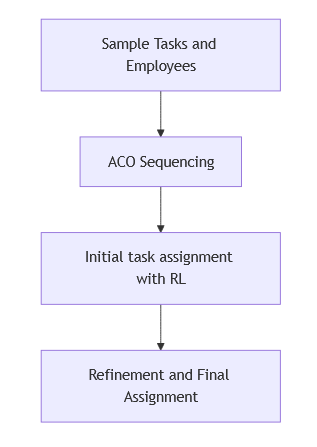
\includegraphics[width=0.3\linewidth]{figures/Initial_flow}
		\caption{\label{fig:flow}Proposed methodology}
	\end{figure}
	
	\section{\label{sec:lit}Literature Survey}
	Reinforcement Learning (RL) has become key for workload optimization and task scheduling in dynamic environments. Ren and Liu \cite{li2024} combined MachineRank with D3QN for schedule adjustment, while Zhang et al. \cite{zhang2022} used PPO for adapting to failures. Infantes et al. \cite{infantes2024} showed GNNs enhance DRL generalization for job-shop scheduling, and Burdett and Kozan \cite{burdett2004} studied limited resource scheduling with heuristic models.
	Zhong \cite{zhong2024} found SARSA provides stable solutions while Q-learning offers higher rewards for task assignment. Ben Noureddine et al. \cite{noureddine2017} applied multi-agent RL for distributed allocation, improving resource usage. Joo et al. \cite{joo2022} developed DRL considering human factors in manufacturing, Wibisono et al. \cite{wibisono2016} recommended real-time worker preference assessment, and Dastmalchian and Blyton \cite{dastmalchian2001} emphasized adaptable scheduling needs.
	Dorigo and Stützle \cite{dorigo2016} reviewed ACO for scheduling problems. Sreyas Ramesh et al. \cite{turn0file0} demonstrated DQN's superiority for energy management. Sivamayil et al. \cite{turn0file1} provided a cross-domain RL review, while Corazza et al. \cite{Corazza2015} compared Q-Learning and SARSA for trading systems.
	This study uses Optuna \cite{Akiba2019Optuna} for hyperparameter optimization and UCB strategy, which Wang et al. \cite{Wang2023TaskScheduling} integrated into QMTSF for cloud scheduling. Sutton and Barto \cite{SuttonBarto1998} provide comprehensive RL algorithm guidance.
	
	\section{\label{sec:problem}Problem Formulation}
	
	In manufacturing and service environments, allocating tasks to a diverse workforce presents a multi-objective challenge. Our methodology integrates bio-inspired optimization, adaptive learning, and post-assignment refinement to maximize successful task assignments while ensuring deadlines are met, workloads are balanced, and skills are effectively utilized.
	
	\subsection{\label{subsec:components}Key Components}
	
	\textbf{Tasks} are characterized by:
	\begin{itemize}
		\item \textbf{Required Skills:} Specific competencies needed for completion.
		\item \textbf{Processing Time:} Estimated hours required.
		\item \textbf{Deadline:} Due date by which the task must be completed.
		\item \textbf{Priority:} Measure of urgency influencing scheduling order.
		\item \textbf{Precedence Constraints:} Dependencies between tasks.
	\end{itemize}
	
	\textbf{Employees} are defined by:
	\begin{itemize}
		\item \textbf{Skill Set:} Collection of competencies.
		\item \textbf{Availability:} Available work hours.
		\item \textbf{Efficiency:} Scaling factor influencing task completion time.
		\item \textbf{Current Workload:} Existing assigned tasks.
	\end{itemize}
	
	\subsection{\label{subsec:strategy}Three-Phase Strategy}
	
	To address this NP-hard scheduling problem, our framework consists of:
	
	\begin{enumerate}
		\item \textbf{Initial Task Sequencing:} Employs bio-inspired optimization (ACO) to generate an initial task ordering based on urgency, processing times, and dependencies.
		
		\item \textbf{Task Assignment through Learning:} A centralized agent dynamically assigns tasks to employees using Q-learning and SARSA algorithms.
		
		\item \textbf{Post-Assignment Refinement:} Iteratively adjusts task-employee mapping to balance workloads and improve skill alignment.
	\end{enumerate}
	
	\section{\label{sec:state}State and Reward Design}
	
	The reinforcement learning state is defined as:
	\begin{equation}
		s = \bigl(i,\,\mathbf{H},\,\mathbf{A},\,\mathbf{F}\bigr)
	\end{equation}
	
	Where $i$ is the task index, $\mathbf{H}$ represents residual work hours, $\mathbf{A}$ tracks assignments, and $\mathbf{F}$ contains task features.
	
	The reward function balances multiple objectives:
	\begin{equation}
		r(s,a) = R_{\text{feas}} + R_{\text{penalty}} + R_{\text{balance}} + R_{\text{efficiency}}
	\end{equation}
	
	\section{\label{sec:algo}Algorithmic Architecture}
	
	Our system integrates:
	
	\begin{enumerate}
		\item \textbf{Ant Colony Optimization (ACO)} for task sequencing, which generates initial sequences considering dependencies, deadlines, and priorities. The probability of transitioning from task $t_i$ to task $t_j$ is computed as:
		\begin{equation}
			p_{ij} = \frac{[\mathbf{P}_{ij}]^{\alpha} \,[\eta_{ij}]^{\beta}}{\sum_{k \in \mathcal{N}_i}[\mathbf{P}_{ik}]^{\alpha} \,[\eta_{ik}]^{\beta}}
		\end{equation}
		where $\mathcal{N}_i$ is the set of candidate tasks for task $t_i$.
		
		\item \textbf{Reinforcement Learning (RL)} for assignment, using both Q-learning:
		\begin{equation}
			Q(s,a) \leftarrow Q(s,a) + \alpha \left[r + \gamma \max_{a'} Q(s',a') - Q(s,a)\right]
		\end{equation}
		and SARSA:
		\begin{equation}
			Q(s,a) \leftarrow Q(s,a) + \alpha \left[r + \gamma Q(s',a') - Q(s,a)\right]
		\end{equation}
		with an $\epsilon$-greedy policy.
		
		\item \textbf{Post-Assignment Refinement} to optimize the initial assignments:
		\begin{equation}
			Q(\mathcal{S},a) \leftarrow Q(\mathcal{S},a) + \alpha_r \left[r + \gamma_r \max_{a'} Q(\mathcal{S}',a') - Q(\mathcal{S},a)\right]
		\end{equation}
	\end{enumerate}
	
	The framework incorporates automated hyperparameter tuning via Optuna to optimize parameters across all stages.
	
	\section{\label{sec:inference}Results and Insights}
	
	Our simulation results demonstrate that:
	
	\begin{itemize}
		\item The combined ACO-RL approach enhances workload balance without compromising assignment rates or deadline compliance.
		
		\item Greedy methods typically overload employees with matching skill profiles, while our RL module redistributes tasks more evenly.
		
		\item The 70:30 epsilon decay schedule with Upper Confidence Bound mechanism improves reward performance by balancing exploration and exploitation.
		
		\item Though the framework improves workload distribution, practical deployment requires careful tuning to align with organizational priorities.
	\end{itemize}
	
	\subsection{\label{subsec:workload}Workload Distribution Insights}
	
	Results indicate that greedy assignment methods typically overload a subset of employees due to repeated allocation of tasks that match their skill profiles. By integrating a workload balancing term into the reward function, the reinforcement learning module gradually redistributes tasks more evenly, as evidenced by a lower standard deviation of assigned hours relative to baseline approaches.
	
	\subsection{\label{subsec:tradeoffs}Practical Trade-offs and Future Considerations}
	
	Although the hybrid ACO-RL framework markedly improves workload distribution, its practical deployment requires careful tuning of reward parameters to align with organizational priorities. Future enhancements could include dynamic adjustment of reward components in response to real-time performance metrics.
	
	The integration of workload balance as a primary objective contributes to more resilient and sustainable workforce management.
	
	\section*{Acknowledgments}
		The authors would like to express their sincere gratitude to SRM Institute of
	Technology for providing the resources and support necessary for this study.
		\nocite{*}
	
	\begin{thebibliography}{99}
		
		
		\bibitem{SuttonBarto1998}
		R.~S. Sutton and A.~G. Barto, \emph{Reinforcement Learning: An Introduction}, MIT Press, 1998.
		
		\bibitem{li2024}
		J. Li, L. Zhang, Z. Li, and S. Zhang, ``Dynamic scheduling for flexible job shop based on MachineRank with deep reinforcement learning,'' \textit{Sci. Rep.}, vol. 14, no. 1, p. 12345, 2024. doi:10.1038/s41598-024-79593-8.
		
		\bibitem{zhang2022}
		M. Zhang, Y. Lu, Y. Hu, N. Amaitik, and Y. Xu, ``Dynamic Scheduling Method for Job-Shop Manufacturing Systems by Deep Reinforcement Learning with Proximal Policy Optimization,'' \textit{Sustainability}, vol. 14, no. 9, p. 5177, 2022. doi:10.3390/su14095177.
		
		
		
		\bibitem{wang2023}
		Wang B, Liu Y, Qian J, Parker SK. The remote revolution: assessing the impact of working from home on employees' productivity and work-life balance. \textit{Future Business Journal}. 2023;9(1):1-14. doi:10.1186/s43093-024-00345-1.
		
		\bibitem{infantes2024} G. Infantes et al., ``Learning to Solve Job Shop Scheduling
		under Uncertainty,'' CPAIOR, 2024.
		
		\bibitem{burdett2004} R. L. Burdett and E. Kozan, ``The Assignment of
		Individual Renewable Resources in Scheduling,'' Asia Pacific Journal of
		Operational Research, 2004.
		
		\bibitem{zhong2024} L. Zhong, ``Comparison of Q-learning and SARSA
		Reinforcement Learning Models on Cliff Walking Problem,'' DAI, 2024.
		
		\bibitem{noureddine2017} D. Ben Noureddine et al., ``Multi-agent Deep Reinforcement
		Learning for Task Allocation in Dynamic Environment,'' ICSOFT, 2017.
		
		\bibitem{joo2022} T. Joo et al., ``Task Allocation in Human–Machine Manufacturing
		Systems Using Deep Reinforcement Learning,'' Sustainability, 2022.
		
		\bibitem{wibisono2016} A. Wibisono, A. S. Nisafani, H. Bae, and Y. Park, ``A dynamic
		and human-centric resource allocation for managing business process execution,''
		University of Texas at El Paso, Tech. Rep., Dec. 2016.
		
		\bibitem{dastmalchian2001} A. Dastmalchian and P. Blyton, ``Workplace flexibility
		and the changing nature of work: An introduction,'' \textit{J. Management Studies},
		vol. 38, no. 2, pp. 281-286, 2001.
		
		\bibitem{dorigo2016} M. Dorigo and T. Stützle, ``Ant colony optimization:
		Overview and recent advances,'' in \textit{Handbook of Metaheuristics}, 3rd
		ed. Springer, 2016, pp. 311-351.
		
		\bibitem{turn0file0} S. Ramesh, S. B. N., S. J. Sathyavarapu, V. Sharma, N. K. A. A., and M. Khanna, ``Comparative analysis of Q-learning, SARSA, and deep Q-network for microgrid energy management,'' \textit{Scientific Reports}, vol. 15, p. 694, 2025, doi:10.1038/s41598-024-83625-8.
		
		\bibitem{turn0file1} K. Sivamayil, E. Rajasekar, B. Aljafari, S. Nikolovski, S. Vairavasundaram, and I. Vairavasundaram, ``A systematic study on reinforcement learning based applications,'' \textit{Energies}, vol. 16, p. 1512, 2023, doi:10.3390/en16031512.
		
		\bibitem{Corazza2015} 
		M. Corazza and A. Sangalli, ``Q-Learning and SARSA: A Comparison between Two Intelligent Stochastic Control Approaches for Financial Trading,'' Working Paper, Ca’ Foscari University of Venice, 2015. Available: \url{https://ssrn.com/abstract=2617630}.
		
		\bibitem{Mavrovouniotis2023} 
		M. Mavrovouniotis, M. N. Anastasiadou, and D. Hadjimitsis, ``Measuring the Performance of Ant Colony Optimization Algorithms for the Dynamic Traveling Salesman Problem,'' \textit{Algorithms}, vol. 16, no. 545, 2023, doi: 10.3390/a16120545. Available: \url{https://doi.org/10.3390/a16120545}.
		
		\bibitem{Akiba2019Optuna} 
		T. Akiba, S. Sano, T. Yanase, T. Ohta, and M. Koyama, \emph{Optuna: A Next-generation Hyperparameter Optimization Framework}, Preprint, compiled July 26, 2019.
		
		
		\bibitem{Wang2023TaskScheduling} 
		Y. Wang, S. Dong, and W. Fan, \emph{Task Scheduling Mechanism Based on Reinforcement Learning in Cloud Computing}, Mathematics, vol. 11, 3364, 2023, doi:10.3390/math11153364.
		
	\end{thebibliography}
	
	\section{\label{sec:appendix}Appendix}
	The source code for this project is available on GitHub at \url{https://github.com/samkrdev/Hybrid-ACO-RL-Task-assigner}.
	
\end{document}